% --- Inference optimisation: KV caching and serving levers ---
\begin{frame}{Where the Serving Memory Goes}
  \begin{columns}[T,onlytextwidth]
    \column{0.52\textwidth}
    \begin{itemize}\footnotesize
      \item[\textcolor{red}{$\blacktriangleright$}] As covered earlier, \textbf{KV caching} keeps the key and value tensors of past positions in GPU memory so decode does not recompute them, at the price of memory that grows with layers, batch size, and context length.
      \item[\textcolor{red}{$\blacktriangleright$}] That memory is the binding constraint in serving: after the weights are loaded, whatever is left is what caps how many requests can run at once.
      \item[\textcolor{red}{$\blacktriangleright$}] Attention variants such as MQA and GQA shrink the cache by sharing key and value heads. The rest of this section attacks the same budget from two other directions: \textbf{how the cache is allocated} (paging) and \textbf{how many bits each entry costs} (quantization).
      \end{itemize}
    \column{0.47\textwidth}
    \centering
    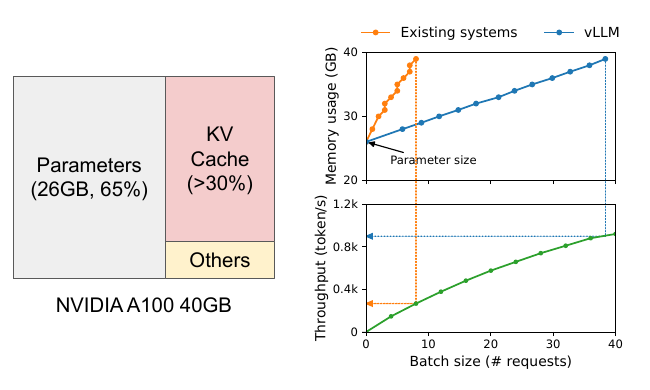
\includegraphics[width=\linewidth,height=0.72\textheight,keepaspectratio]{images/inference-optimisation/vllm_paper_fig1_a100_memory_layout.png}\\[-0.1em]
    {\scriptsize Serving a 13B model on an NVIDIA A100 (40\,GB): weights take 65\% of memory, the KV cache over 30\%. Kwon et al., \href{https://arxiv.org/abs/2309.06180}{arXiv:2309.06180}, Figure 1.}
  \end{columns}
\end{frame}

\begin{frame}{Batching: Static vs.\ Continuous}
  \begin{itemize}\itemsep0.5em
    \item[\textcolor{red}{$\blacktriangleright$}] A single decode stream is a matrix-vector workload that leaves most of the GPU idle; batching many requests turns it back into matrix-matrix work.
    \item[\textcolor{red}{$\blacktriangleright$}] \textbf{Static batching:} requests are grouped up front and the whole batch runs until its longest member finishes; short requests hold their slot while doing nothing.
    \item[\textcolor{red}{$\blacktriangleright$}] \textbf{Continuous batching:} scheduling happens per decode step; finished sequences leave the batch immediately and waiting requests join mid-flight. Introduced as \textbf{iteration-level scheduling} by Orca (Yu et al., 2022) and later popularised under the name continuous batching.
    \item[\textcolor{red}{$\blacktriangleright$}] Standard in modern serving stacks (vLLM, TensorRT-LLM, TGI): large throughput gains with no change to model outputs.
  \end{itemize}
\end{frame}

\begin{frame}{KV Cache Fragmentation}
  \begin{itemize}\itemsep0.3em
    \item[\textcolor{red}{$\blacktriangleright$}] Early serving systems stored each request's KV cache as one contiguous tensor, allocated up front for the maximum possible sequence length.
    \item[\textcolor{red}{$\blacktriangleright$}] Three kinds of waste follow: reserved slots not yet used, internal fragmentation (slots never used because the request ends early), and external fragmentation between buffers.
    \item[\textcolor{red}{$\blacktriangleright$}] Measured effective KV memory utilisation in such systems can drop to about 20\%.
  \end{itemize}
  \centering
  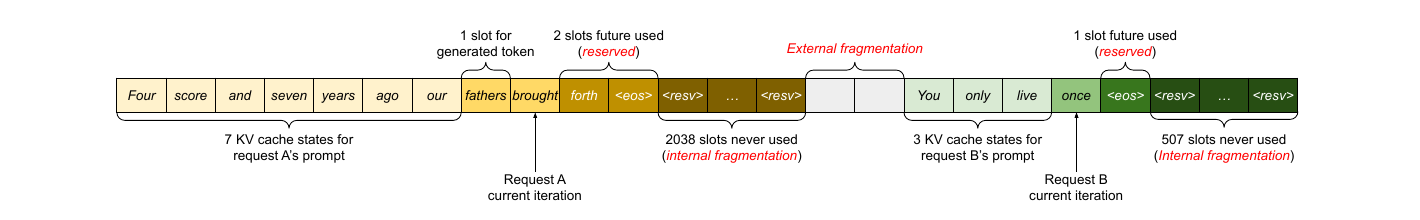
\includegraphics[width=\textwidth,height=0.34\textheight,keepaspectratio]{images/inference-optimisation/vllm_paper_fig3_kv_cache_fragmentation.png}\\[0.15em]
  {\scriptsize Kwon et al., ``Efficient Memory Management for Large Language Model Serving with PagedAttention,'' \href{https://arxiv.org/abs/2309.06180}{arXiv:2309.06180}, Figure 3.}
\end{frame}

\begin{frame}{PagedAttention (vLLM)}
  \begin{itemize}\itemsep0.3em
    \item[\textcolor{red}{$\blacktriangleright$}] Borrow virtual memory from operating systems: split each request's KV cache into fixed-size blocks and allocate blocks on demand.
    \item[\textcolor{red}{$\blacktriangleright$}] A block table maps logical positions to physical blocks, so the cache no longer needs to be contiguous; waste is limited to the last partially filled block, and blocks can be shared across sequences (parallel sampling, shared prefixes).
    \item[\textcolor{red}{$\blacktriangleright$}] vLLM built on this achieves 2--4$\times$ the throughput of prior serving systems at the same latency.
  \end{itemize}
  \centering
  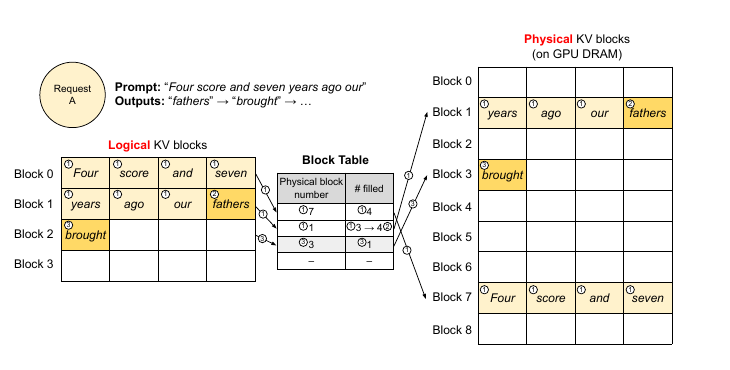
\includegraphics[width=0.58\textwidth,height=0.4\textheight,keepaspectratio]{images/inference-optimisation/vllm_paper_fig6_block_table_paging.png}\\[0.15em]
  {\scriptsize Block table translation. Kwon et al., \href{https://arxiv.org/abs/2309.06180}{arXiv:2309.06180}, Figure 6.}
\end{frame}

\begin{frame}{Speculative Decoding: The Idea}
  \begin{itemize}\itemsep0.5em
    \item[\textcolor{red}{$\blacktriangleright$}] Decode is memory-bound: for the large model, scoring $K$ proposed tokens in one forward pass costs about the same as generating a single token.
    \item[\textcolor{red}{$\blacktriangleright$}] A small \textbf{draft model} proposes $K$ tokens autoregressively; the large \textbf{target model} then evaluates all $K$ positions in parallel.
    \item[\textcolor{red}{$\blacktriangleright$}] Accept draft tokens while they are consistent with the target distribution; at the first rejection, resample that token from an adjusted distribution and discard the rest.
    \item[\textcolor{red}{$\blacktriangleright$}] The output distribution is provably identical to decoding with the target model alone; the speed comes from accepting several tokens per target pass.
    \item[\textcolor{red}{$\blacktriangleright$}] Reported speedups with no change to the output distribution: 2--3$\times$ on T5-XXL (Leviathan et al., 2023) and 2--2.5$\times$ on Chinchilla 70B (Chen et al., 2023).
  \end{itemize}
\end{frame}

\begin{frame}{Speculative Decoding: The Acceptance Rule}
  \begin{itemize}\itemsep0.3em
    \item[\textcolor{red}{$\blacktriangleright$}] Write $q$ for the target model's next-token distribution and $p$ for the draft model's. For each proposed token $\tilde{x}$, draw $r \sim U[0,1]$ and \textbf{accept} it when
      \[
        r < \min\!\left(1,\ \frac{q(\tilde{x} \mid x_{1:n})}{p(\tilde{x} \mid x_{1:n})}\right).
      \]
    \item[\textcolor{red}{$\blacktriangleright$}] So a token the target likes at least as much as the draft does is always accepted; one the draft over-proposed is accepted only in proportion $q/p$.
    \item[\textcolor{red}{$\blacktriangleright$}] On the first rejection, the remaining proposals are discarded and that position is resampled from the \textbf{residual} distribution $\big(q(x \mid x_{1:n}) - p(x \mid x_{1:n})\big)_{+}$, renormalised, where $(f)_{+} = \max(0, f)$. This is what makes the accept/reject step exact rather than an approximation.
    \item[\textcolor{red}{$\blacktriangleright$}] If all $K$ proposals are accepted, one extra token is sampled from the target's own distribution, so a single target pass can yield up to $K+1$ tokens.
  \end{itemize}
  \vspace{0.1em}
  {\scriptsize Modified rejection sampling, Algorithm 2 and Theorem 1 of Chen et al., ``Accelerating Large Language Model Decoding with Speculative Sampling,'' \href{https://arxiv.org/abs/2302.01318}{arXiv:2302.01318}.}
\end{frame}

\begin{frame}{Speculative Decoding: Acceptance in Practice}
  \centering
  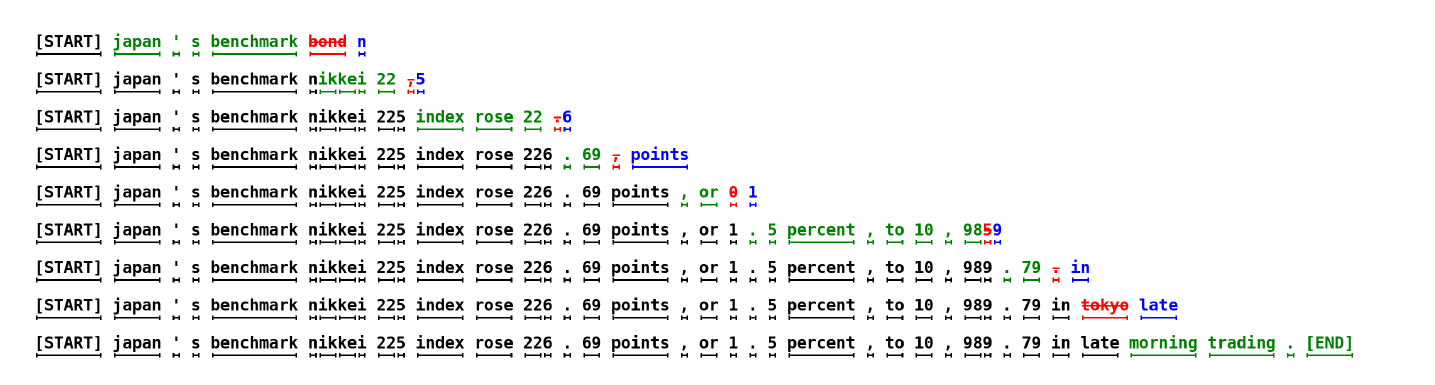
\includegraphics[width=\textwidth,height=0.5\textheight,keepaspectratio]{images/inference-optimisation/leviathan_speculative_decoding_accepted_tokens.png}\\[0.3em]
  \begin{itemize}\footnotesize\itemsep0.2em
    \item[\textcolor{red}{$\blacktriangleright$}] Each line is one iteration: green tokens were proposed by the draft model and accepted, red were rejected, and blue are the target model's corrections.
    \item[\textcolor{red}{$\blacktriangleright$}] This 38-token sentence needed only 9 serial passes of the target model.
    \item[\textcolor{red}{$\blacktriangleright$}] Gains are largest when the draft agrees with the target on the easy tokens, which is most of them.
  \end{itemize}
  {\scriptsize Leviathan, Kalman \& Matias, ``Fast Inference from Transformers via Speculative Decoding,'' \href{https://arxiv.org/abs/2211.17192}{arXiv:2211.17192}, Figure 1.}
\end{frame}

\begin{frame}{Other Inference Levers}
  \begin{itemize}
    \item[\textcolor{red}{$\blacktriangleright$}] \textbf{Kernel fusion \& IO-aware attention} (e.g.\ FlashAttention-style): reduce HBM traffic.
    \item[\textcolor{red}{$\blacktriangleright$}] \textbf{Prefix caching:} reuse the KV cache of shared prompt prefixes (system prompts, few-shot examples) across requests.
    \item[\textcolor{red}{$\blacktriangleright$}] \textbf{Weight sharing / low-rank adapters (LoRA):} smaller footprints where applicable.
    \item[\textcolor{red}{$\blacktriangleright$}] \textbf{Approximate attention} (long contexts): trade accuracy for sub-quadratic cost.
  \end{itemize}
\end{frame}
